\documentclass[9pt,twocolumn,twoside]{pnas-report}

\templatetype{pnasresearcharticle}

\usepackage{lipsum}

\title{Title of a Project}

\author[a,1]{Fine Author}
\author[a,b]{Another Author} 
\author[b]{Other Fine Authors}

\affil[a]{University of Ljubljana, Faculty of Computer and Information Science, Ve\v{c}na pot 113, SI-1000 Ljubljana, Slovenia}
\affil[b]{Other Fine Institutions}

\leadauthor{Author} 

\authordeclaration{All authors contributed equally to this work.}
\correspondingauthor{\textsuperscript{1}To whom correspondence should be addressed. E-mail: fine.author@email.com.}

\begin{abstract}
We study a phenomenon that we claim is important in a subject in which we claim many people are interested. We also claim that such ideas have been studied heavily both in network science and in other disciplines, although all prior work on this topic is horrible (though we will try to phrase that statement as politely as possible). One particular idea, which has some intriguing features but which either rarely has been studied or has only been studied in a crappy way before, is the one that we investigate in this project. Invoking minimal sarcasm, we study an extended version of this idea with our new approach, which we will claim to give universal results if we can get away with it. Our new approach has some bells and whistles that we study in our project, and we use computations, theory, and experiments to give important insights into a phenomenon that many people care about. We also give some gratuitous caveats so that peers will take us seriously, and we pray to our favorite deity that this approach is not equivalent to one that already exists (we forgot to check, and the authors need to graduate). We hope that our study, in addition to its intrinsic quality, will inspire future investigations, citations, and successful grants (and --- who knows? --- maybe even a Turing Award). In case you did not see it last time, we claim once again that our approach is universal.
\end{abstract}

\dates{The manuscript was compiled on \today}
\doi{\href{https://ucilnica.fri.uni-lj.si/course/view.php?id=183}{Introduction to Network Analysis} 2020/21}

\begin{document}

\maketitle
\thispagestyle{firststyle}
\ifthenelse{\boolean{shortarticle}}{\ifthenelse{\boolean{singlecolumn}}{\abscontentformatted}{\abscontent}}{}

\dropcap{P}{\bf roblem definition, motivation, background and contributions.}
\lipsum[1-5]


\dropcap{A}{\bf ssociation football is the world's most popular sport.} During gameplay, players attempt to create goal-scoring opportunities through various methods of individual control of the ball. While these can include dribbling, tackling and taking direct shots, the most common one is passing the ball to a teammate. Progressing the ball along the pitch with a series of passes helps the team retain control of the match, enabling them to realize set plays. It is worth noting that this method is not only common, but also effective, as exhibited by the correlation of per-game average pass frequency and overall tea, success. \cite{plpasses}

Ball movement and goal-scoring opportunities in a football match are complex phenomena to model. Pass characteristics, such as their length, speed or the involved players' positions are often used to provide further insights into their importance and quality. Logging such characteristics for hundreds of passes that happen in any given football match, however, renders the resulting data structure very complex and hard to interpret. To infer more general information about longer stints of play, simpler arrangements, such as networks with player nodes and directed pass links, should be considered.

There are several events in any given football match, that might incur a fundamental change in a team's tactics and approach towards the game. The coaching staff might recognize weak points in the opposition's strategy and relay them to the players during half-time. Suddenly conceding a goal in a must-win game might prompt a team to take more risks and try a different approach, while we can often observe leading teams resort to time-wasting tactics to ensure their victory. 

I
In this project proposal, we introduce several hypotheses for novel ways of match analysis. By using methods of measuring change in team pass map centrality, by observing alterations of its underlying communities and by recognizing the (dis)appearance of distinct player graphlets as a result of a key event in a football match, we plan to study common team behaviours that said events might induce. We recognize these insights as useful in several areas. First, they serve as a form of establishing several ground truths about common trends of play, that might underpin further research. Secondly, more fine-grained difference of successful and unsuccessful responses to key events might be observed and be used in match preparations by domain experts. Finally, we recognize real-time applications of the proposed methods as useful in broadcasting, betting, commentary and analytics, to name only a few fields.


\begin{figure}[t]\centering%
	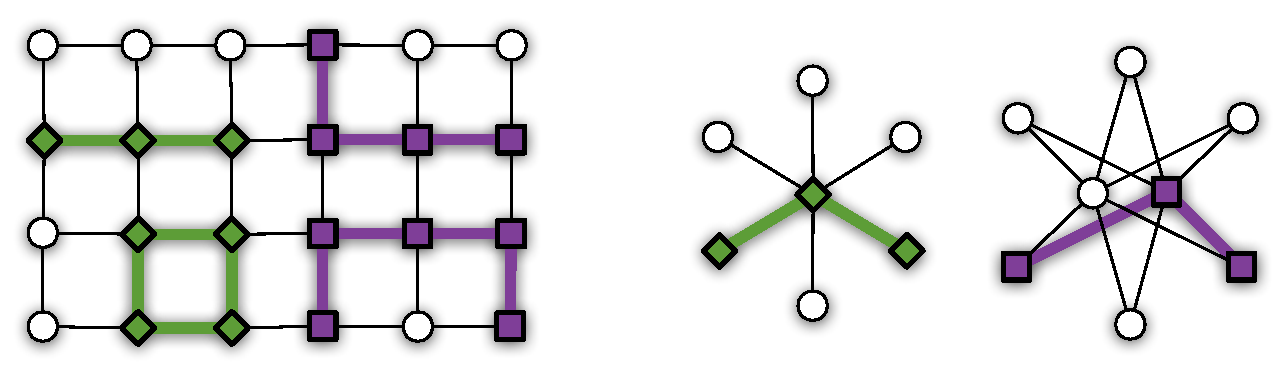
\includegraphics[width=0.8\linewidth]{examples}
	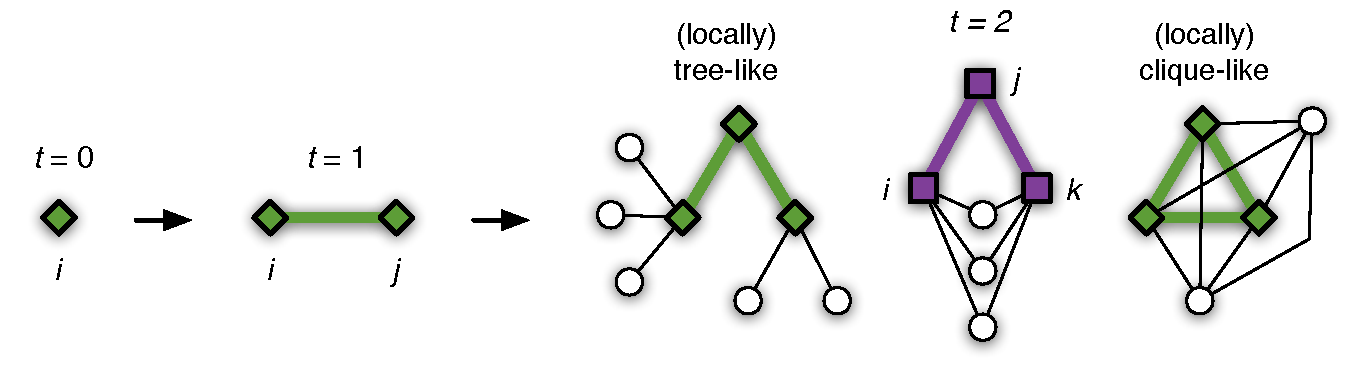
\includegraphics[width=\linewidth]{growth}
	\caption{Mandatory informative illustration highlighting main contributions.~\cite{Sub18a}}
	\label{fig:example}
\end{figure}

\section*{Related work}

{\bf Selected relevant literature ($\approx 15$ references).}
\lipsum[1-3]

\nocite{Kle00,Bou05,EB07,New08,For10,New12,FH16,PLC17,PDL18,Pei20}

\section*{Results}

\begin{table}[t]\centering%
	\caption{Table describing data or methods.}
	\begin{tabular}{lccccc}\toprule
	    & $n$ & $m$ & $\langle k\rangle$ & $\langle C\rangle$ & $\langle d\rangle$ \\\midrule
	    Fine network & $438\,920$ & $9\,742\,733$ & $44.4$ & $0.37$ & $6.19$ \\
	    Random graph & $438\,920$ & $9\,781\,609$ & $44.6$ & $0.00$ & $4.92$ \\\bottomrule
	\end{tabular}
	\label{tbl:example}
\end{table}

{\bf Main results supported by plots, figures, tables, diagrams etc.}
\lipsum[1-2]

\begin{figure}[h]\centering%
	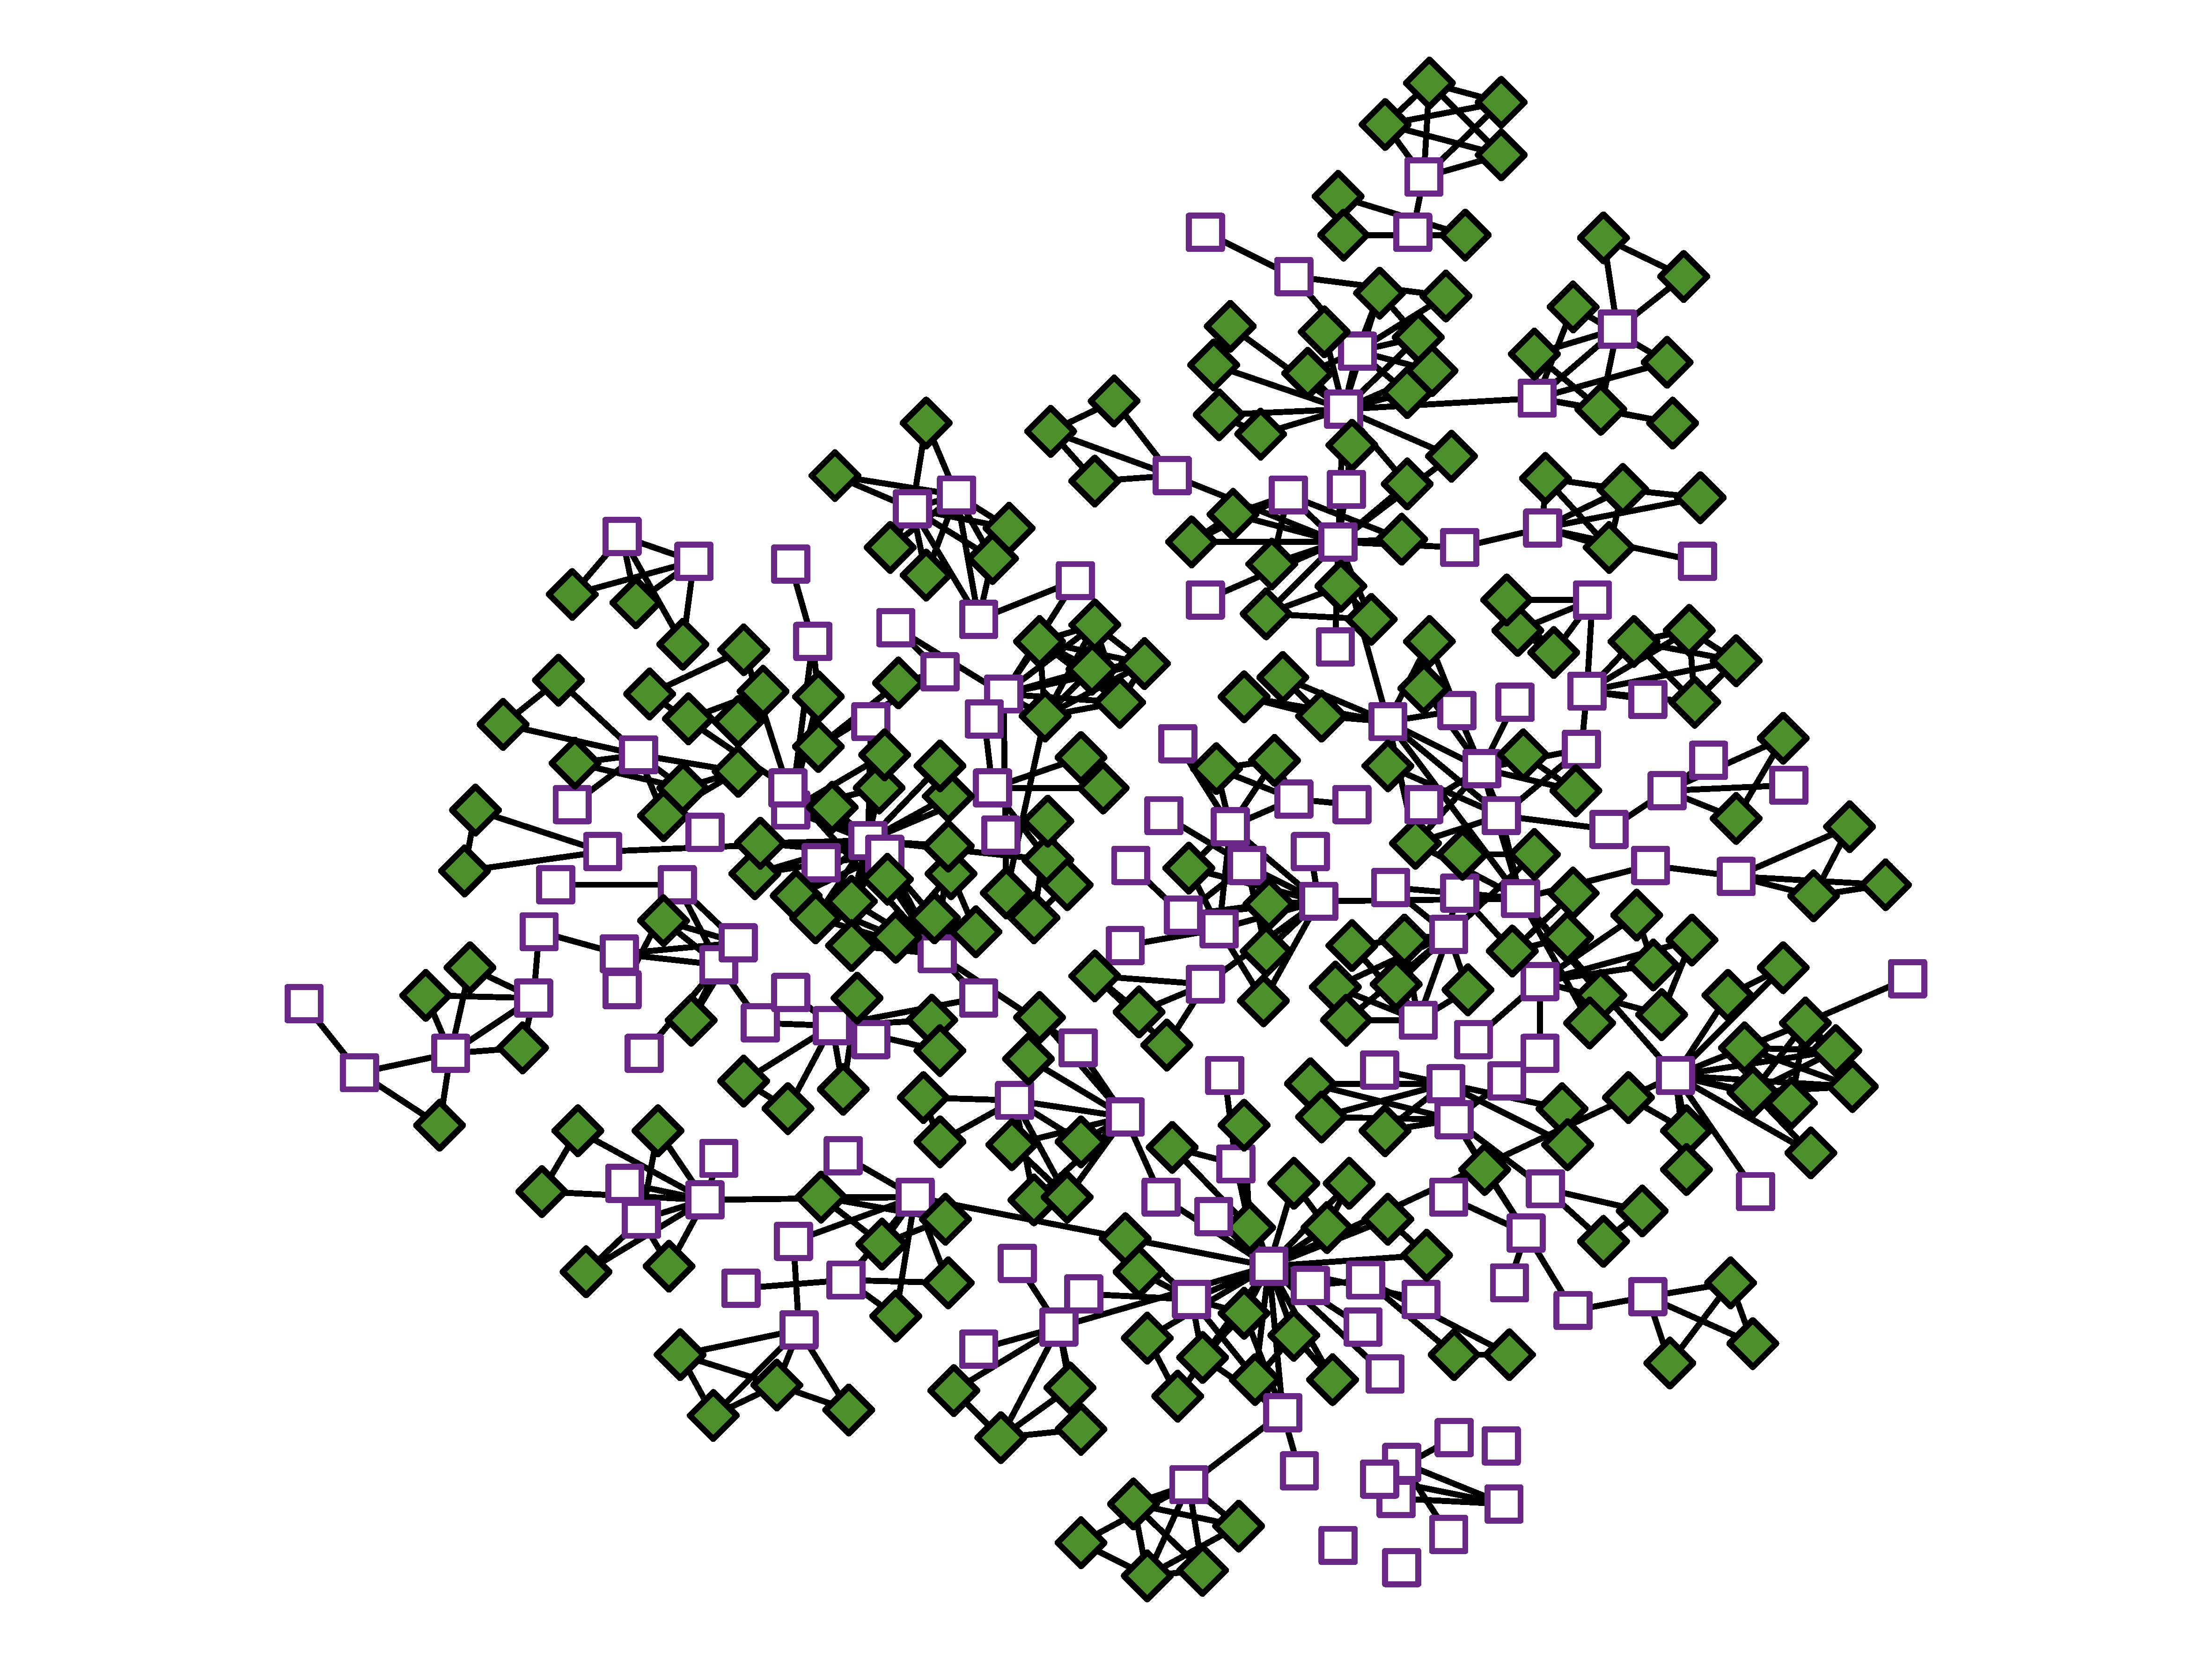
\includegraphics[width=0.49\linewidth]{example1}
	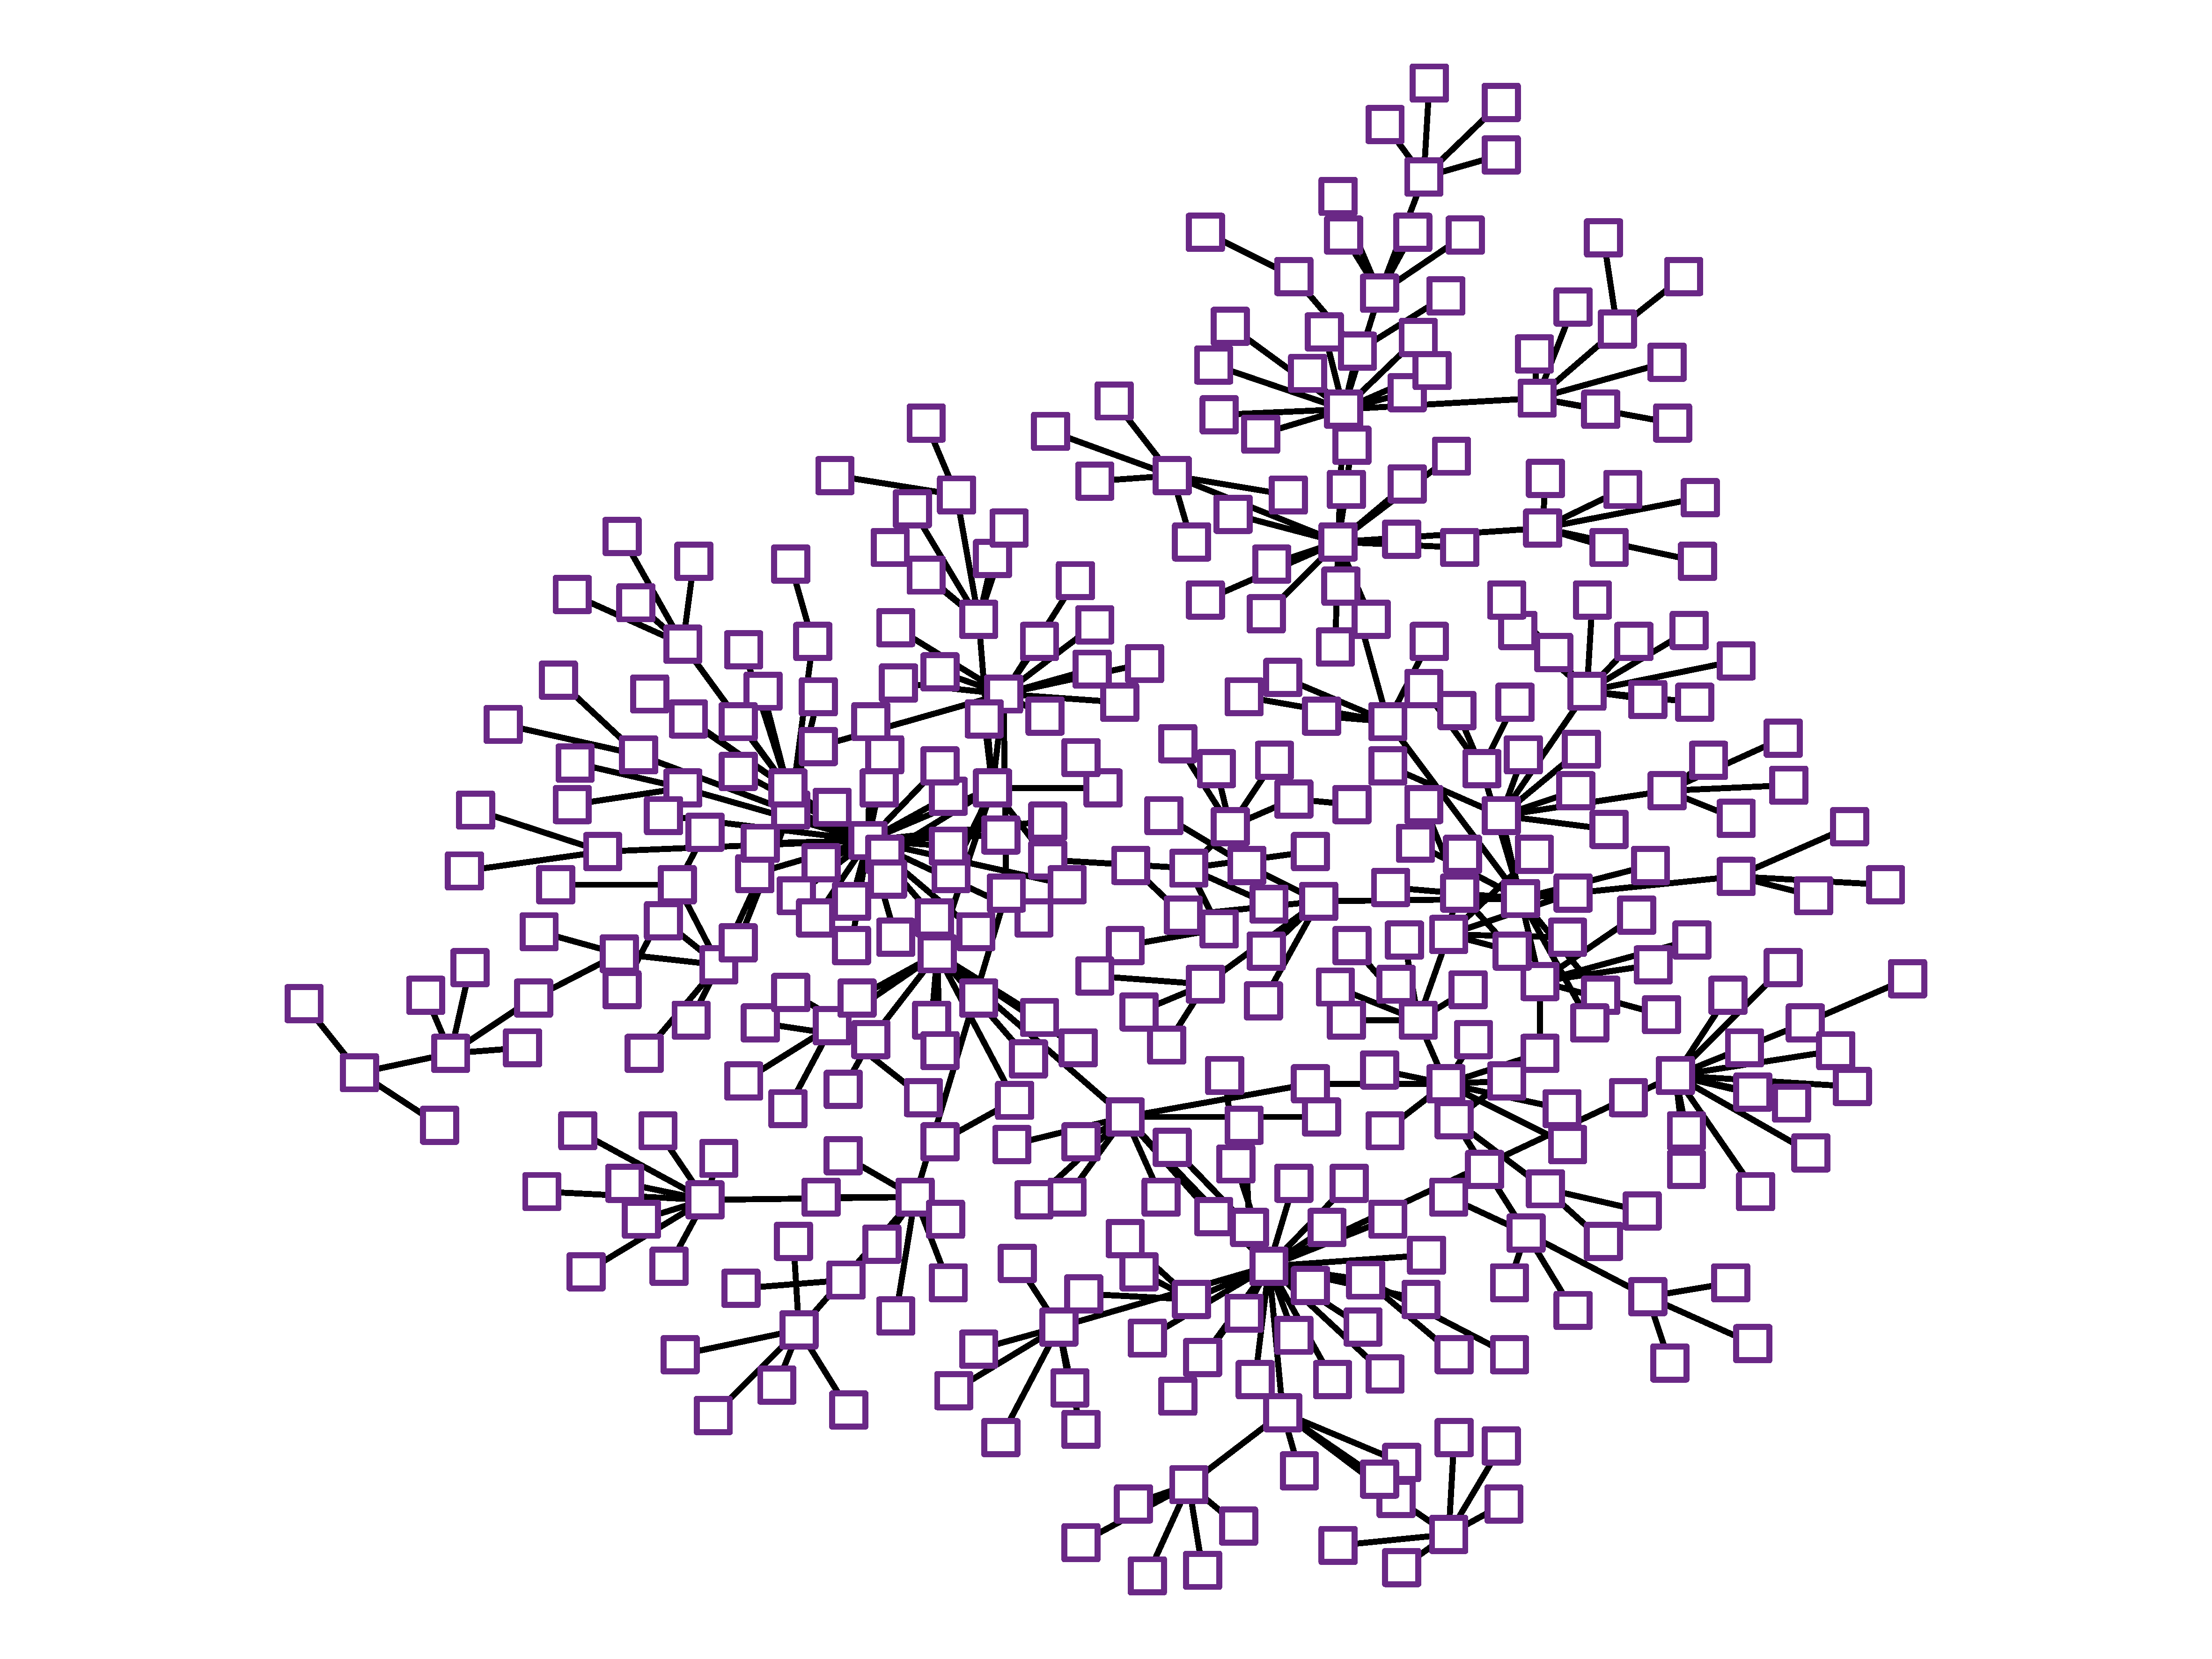
\includegraphics[width=0.49\linewidth]{example2}
	\caption{Figure showing interesting examples.~\cite{Sub18a}}
\end{figure}

\lipsum[3-8]

\begin{figure}[t]\centering%
	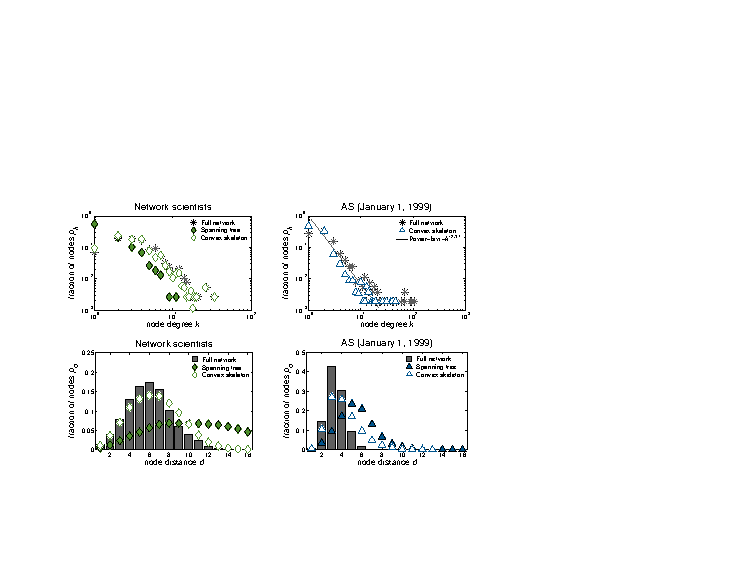
\includegraphics[width=\linewidth]{distributions}
	\caption{Figure showing relevant results.~\cite{Sub18a}}
\end{figure}

\begin{figure}[b]\centering%
	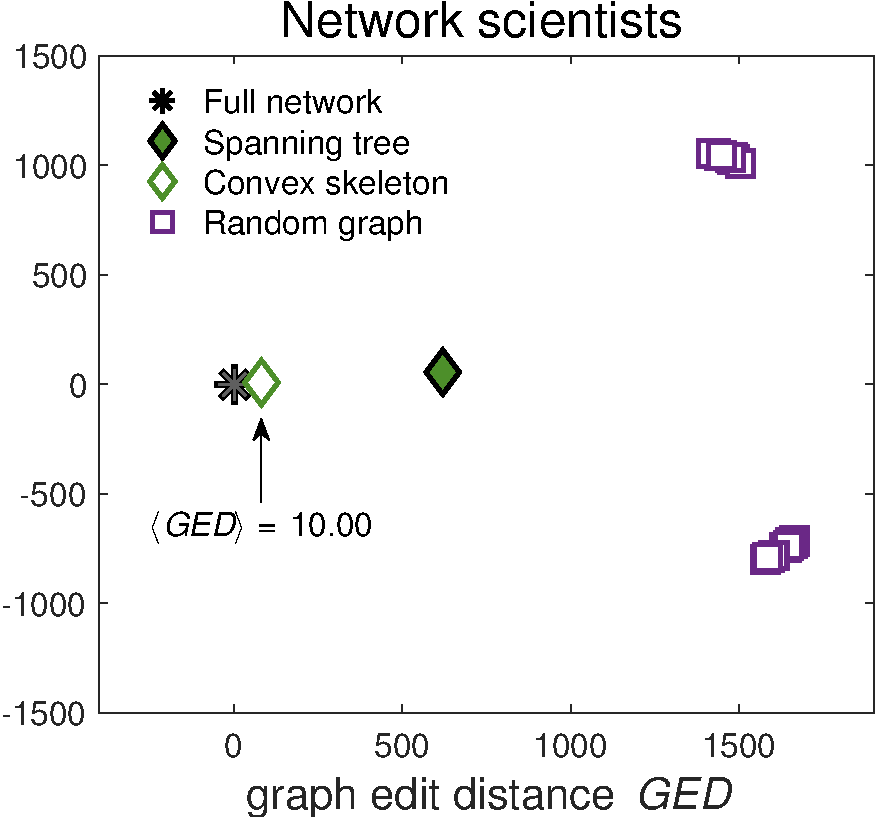
\includegraphics[width=0.45\linewidth]{results1}\hskip12pt
	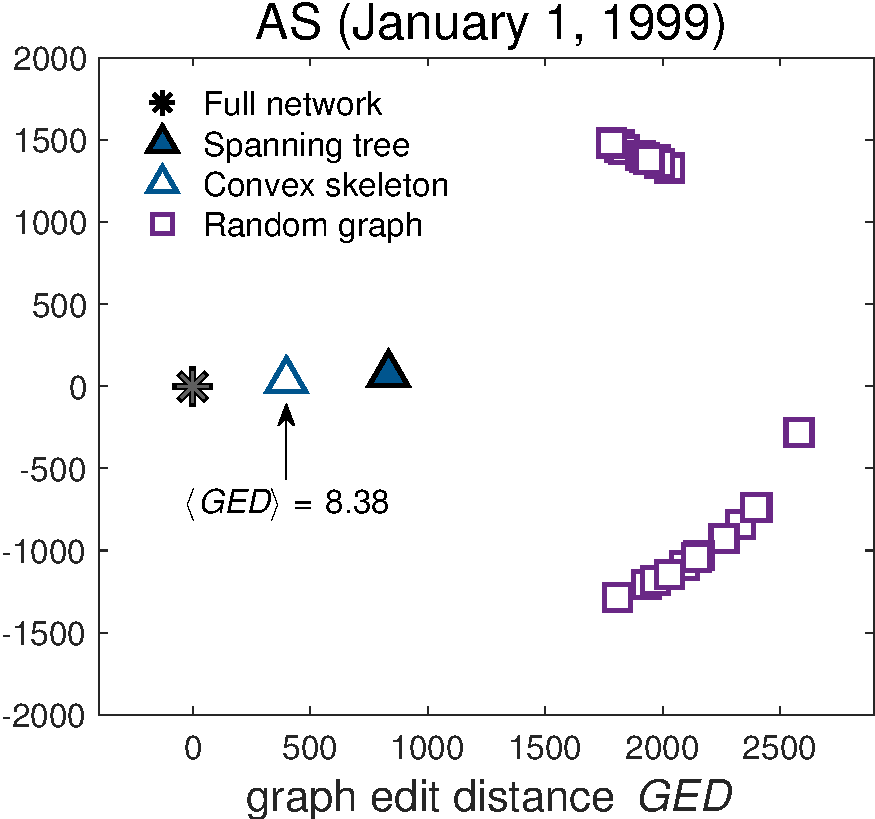
\includegraphics[width=0.45\linewidth]{results2}
	\caption{Another figure with results.~\cite{Sub18a}}
	\label{fig:example}
\end{figure}

\section*{Discussion}

{\bf Discussion of results, main contributions, final conclusions and future work.}
\lipsum[1-5]

{\small\section*{Methods}

{\bf Describe data, methods and algorithms (use subsections).}
\lipsum[1-3]
\begin{equation}
	\phi_v = \Pr(X_{st}(v) = 1) = \Pr(X_{sv} = 1)\Pr(X_{vt} = 1)
	\label{eq:example}
\end{equation}

\lipsum[4-5]}

\acknow{The authors would like to\dots}

\showacknow{}

\bibliography{bibliography}

\end{document}